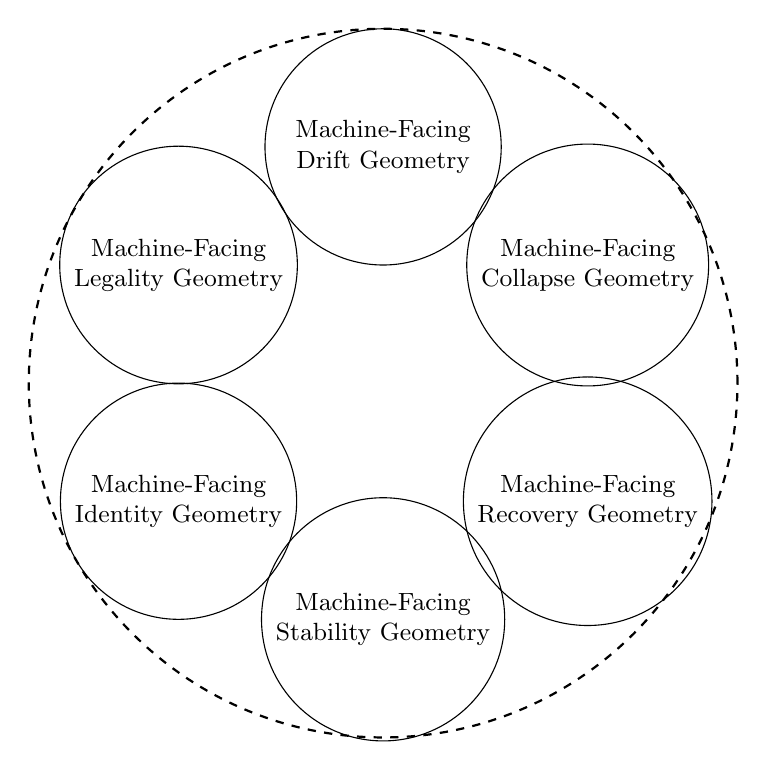
\begin{tikzpicture}[
    plane/.style={circle, draw, minimum size=3cm, align=center, font=\small},
    field/.style={rectangle, draw, rounded corners=4pt, minimum width=2cm, minimum height=0.8cm, font=\scriptsize}
]

\node[plane] (drift) at (90:3) {Machine-Facing\\Drift Geometry};
\node[plane] (collapse) at (30:3) {Machine-Facing\\Collapse Geometry};
\node[plane] (recovery) at (-30:3) {Machine-Facing\\Recovery Geometry};
\node[plane] (stability) at (-90:3) {Machine-Facing\\Stability Geometry};
\node[plane] (identity) at (-150:3) {Machine-Facing\\Identity Geometry};
\node[plane] (legality) at (150:3) {Machine-Facing\\Legality Geometry};

\draw[thick, dashed] circle (4.5cm);

\end{tikzpicture}

